% This text is proprietary.
% It's a part of presentation made by myself.
% It may not used commercial.
% The noncommercial use such as private and study is free
% Sep. 2005 
% Author: Sascha Frank 
% University Freiburg 
% www.informatik.uni-freiburg.de/~frank/


\documentclass{beamer}
\usepackage{graphicx}
\usepackage{amsmath}
\usepackage{amssymb}
\usepackage{xcolor}
\definecolor{mygreen}{cmyk}{0.82,0.11,1,0.25}
\begin{document}
\title{Spring 2020 MAT303 Recitations}   
\author{Week of 4/20/20: Sections 4.1 and 4.2} 
\date{} 

\frame{\titlepage} 


\frame{\frametitle{Section 4.1: First-order systems and applications}

A system of differential equation consists of a finite collection of differential equations in indeterminates $x_1(t), x_2(t), \cdots, x_n(t)$, depending on a parameter $t$. In this chapter, we will deal with linear systems. \pause

One's first encounter wiht systems of differential equations arises from higher-order scalar equations. One way of solving them is by reducing such equations to systems of first-order problems, as we shall see next. . 
}

\frame{\frametitle{Section 4.1: First-order systems and applications}
This example is extracted from problem 4.1.3 in our textbook. Consider the third-order equation
\begin{equation*}
tx^{(3)}-2t^2x^{''}+3tx^{'}+5x=\ln(t)
\end{equation*}
By using the substitutions $x_1=x$, $x_2=x^{'}$, $x_3=x^{''}$, we can rewrite this equation as a system in three variables
\begin{align*}
tx_{3}^{'}-2t^2x_3+3tx_2+5x_1 & = \ln(t) \\
x_{2}^{'} & = x_3\\
x_1^{'} & = x_2
\end{align*}

}

\frame{\frametitle{Section 4.1: First-order systems and applications}
The following example is extracted from problem 4.1.17. \pause Consider the system of differential equations
\begin{align*}
x^{'} & = y \\
y^{'} & = -x
\end{align*}
\pause
By elimination, we find
\begin{equation*}
x^{''} = y^{'} = -x.
\end{equation*}
\pause
This second-order equation on $x$ can be solved by the method of characteristic equations, 
\begin{equation*}
x(t)=A\cos(t)+B\sin(t).
\end{equation*}
\pause
}

\frame{\frametitle{Section 4.1: First-order systems and applications}
To solve for $y$, we use the first equation in our system,  
\begin{align*}
y (t) & = x'(t) \\
& = -A\sin(t)+B\cos(t).
\end{align*}
\pause
Below is a plot of the slope field for this equation, with several solution curves outlined. 
\begin{center}
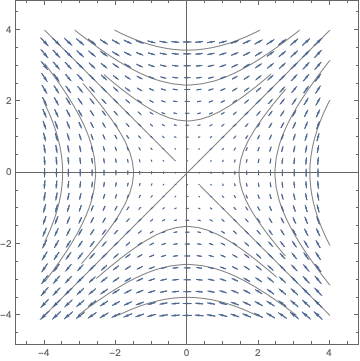
\includegraphics[width=0.5\textwidth]{p4.png} 
\end{center}
}

\frame{\frametitle{Section 4.1: First-order systems and applications}
In this example, extracted from problem 4.1.23, we have the system
\begin{align*}
x^{'} & = y \\
y^{'} & = 6x-y,
\end{align*}
\pause
with initial conditions $x(0=1$, $y(0)=2$. \pause We can turn this system into a second-order equation for $x$ as follows, 
\begin{equation*}
x^{''} = y^{'} = 6x-y = 6x-x^{'}, 
\end{equation*}
\pause
that is
\begin{equation*}
x^{''}+x^{'}-6x=0.
\end{equation*}
\pause
The characteristic polynomail of this equation is $r^2+r-6r=(r-2)(r+3)$, with roots $r=2, r=-3$.  The general solution takes the form
\begin{equation*}
x(t)=Ae^{2t}+Be^{-3t}
\end{equation*}
}

\frame{\frametitle{Section 4.1: First-order systems and applications}
To find the appropriate values for the constants, we need to set up the intial conditions in terms of $x$. \pause The initial condition on $y$ yields 
\begin{equation*}
x^{'}(0) = y(0) = 2,
\end{equation*}
\pause
thus we find
\begin{align*}
A+B & = 1\\
2A-3B & = 2,
\end{align*}
\pause
whose solutions are $A=1, B=0$. \pause As a result, $x(t)=e^{2t}$, and 
\begin{equation*}
y(t) = x^{'}(t) = 2e^{2t}
\end{equation*}
}

\frame{\frametitle{Section 4.1: First-order systems and applications}
Below is a plot of the direction field, as well as the solution curve corresponding to the given initial condition (in red).
\begin{center}
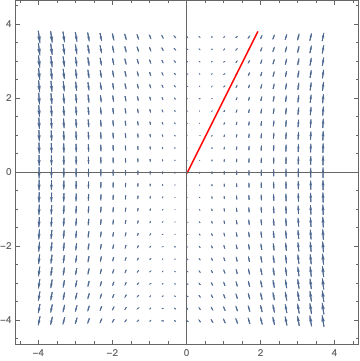
\includegraphics[width=0.5\textwidth]{p5.png} 
\end{center}
}


\frame{\frametitle{Section 4.2: The method of elimination}
Consider the following system, extracted from problem 4.2.5, 
\begin{align*}
x^{'} & = -3x-4y \\
y^{'} & = 2x+y.
\end{align*}
\pause
We will rewrite the system by using the short-hand notation $D$ to mean derivatives relative to time, $D=\frac{d}{dt}$, 
\begin{align*}
(D+3)x+4y & = 0\\
-2x + (D-1)y & = 0
\end{align*}
\pause
In order to eliminate one of the variables from the system, we will perform the following operations:
\begin{enumerate}
\item Apply the operator $(D-1)$ to the first equation, that is, differentiate it and subtract the original equation from the result.
\pause
\item Multiply the second equation by $(-4)$. 
\end{enumerate}
\pause
}

\frame{\frametitle{Section 4.2: The method of elimination}
The resulting (equivalent) system is 
\begin{align*}
(D-1)(D+3)x+4(D-1)y & = 0\\
8x -4 (D-1)y & = 0
\end{align*}
\pause
By adding the two equations we find
\begin{equation*}
(D-1)(D+3)x + 8x =0,
\end{equation*}
which in usual notation for derivatives is 
\begin{align*}
(D-1)(D+3)x + 8x & =0\\
(D-1)(x^{'}+3x)+8x & = 0\\
(x^{'}+3x)^{'}-(x^{'}+3x)+8x & = 0\\
x^{''}+3x^{'}-x^{'}-3x+8x & = 0\\
x^{''}+2x^{'}+5x & = 0
\end{align*}
}

\frame{\frametitle{Section 4.2: The method of elimination}
This equation can be solved bby the method of characteristic equations, and I will leave the details to you. Its solutions take the form
\begin{equation*}
x(t)=e^{-t}(A\cos(2t)+B\sin(2t)).
\end{equation*}
\pause
To find the solution $y(t)$ we may use the first equation of the system,
\begin{align*}
y(t) & = -\frac{x^{'} +3x}{4} \\
& =-\frac{e^{-t}[(2B-A)\cos(2t) -(2A+B)\sin(2t)]+3e^{-t}(A\cos(2t)+B\sin(2t))}{4} \\
& = -\frac{e^{-t}[(A+B)\cos(2t)+(B-A)\sin(2t)]}{2}
\end{align*}
}
%
%\section{Section no.3} 
%\subsection{Tables}
%\frame{\frametitle{Tables}
%\begin{tabular}{|c|c|c|}
%\hline
%\textbf{Date} & \textbf{Instructor} & \textbf{Title} \\
%\hline
%WS 04/05 & Sascha Frank & First steps with  \LaTeX  \\
%\hline
%SS 05 & Sascha Frank & \LaTeX \ Course serial \\
%\hline
%\end{tabular}}
%
%
%\frame{\frametitle{Tables with pause}
%\begin{tabular}{c c c}
%A & B & C \\ 
%\pause 
%1 & 2 & 3 \\  
%\pause 
%A & B & C \\ 
%\end{tabular} }
%
%
%\section{Section no. 4}
%\subsection{blocs}
%\frame{\frametitle{blocs}
%
%\begin{block}{title of the bloc}
%bloc text
%\end{block}
%
%\begin{exampleblock}{title of the bloc}
%bloc text
%\end{exampleblock}
%
%
%\begin{alertblock}{title of the bloc}
%bloc text
%\end{alertblock}
%}
\end{document}


